\title{%
  Git version control
}
\author{Daniel Bosk}
\institute{%
  KTH EECS
}

\mode<article>{\maketitle}
\mode<presentation>{%
  \begin{frame}
    \maketitle
  \end{frame}
}

\mode*

\begin{abstract}
  % What's the problem?
% Why is it a problem? Research gap left by other approaches?
% Why is it important? Why care?
% What's the approach? How to solve the problem?
% What's the findings? How was it evaluated, what are the results, limitations, 
% what remains to be done?

% XXX Summary
\emph{Summary:}
\dots

% XXX Motivation and intended learning outcomes
\emph{Intended learning outcomes:}
\dots

% XXX Prerequisites
\emph{Prerequisites:}
\dots

% XXX Reading material
\emph{Reading:}
\dots

\end{abstract}


\begin{frame}
  \centering
  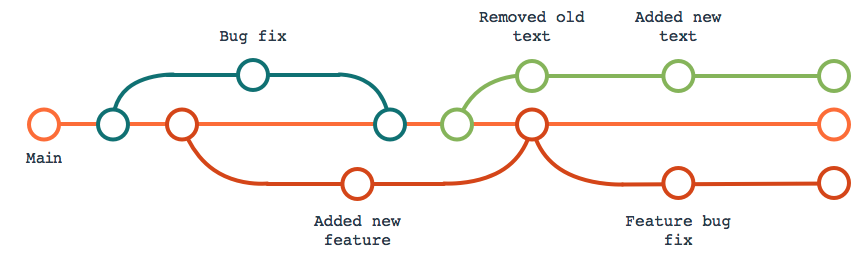
\includegraphics[width=\columnwidth]{figs/version-tree.png}
\end{frame}


\section{What's the problem?}

\subsection{The problem}

\begin{frame}
  \begin{question}
    \begin{itemize}
      \item How to manage project files?
      \item During development?
      \item Future revisions?
    \end{itemize}
  \end{question}
\end{frame}

\subsection{Common solutions}

\begin{frame}
  \begin{alertblock}{Solutions}
    \begin{itemize}
      \item Dropbox
      \item \enquote{report-final-version}, 
        \enquote{report-final-final-version}, \dots
      \item \enquote{report-20200828}
    \end{itemize}
  \end{alertblock}

  \pause

  \begin{remark}
    \begin{itemize}
      \item It works \dots
    \end{itemize}
  \end{remark}
\end{frame}


\section{Our solution}

\subsection{Version management}

\begin{frame}
  \centering
  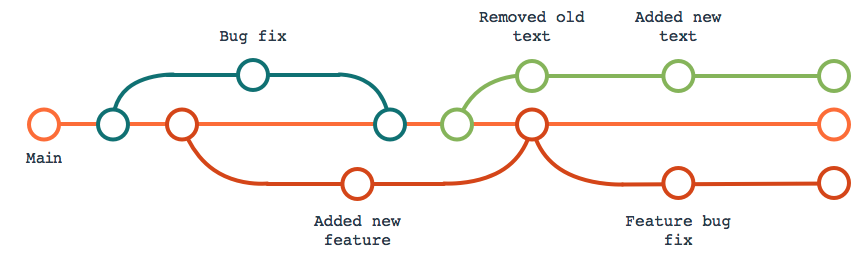
\includegraphics[width=\columnwidth]{figs/version-tree.png}
\end{frame}

\begin{frame}
  \centering
  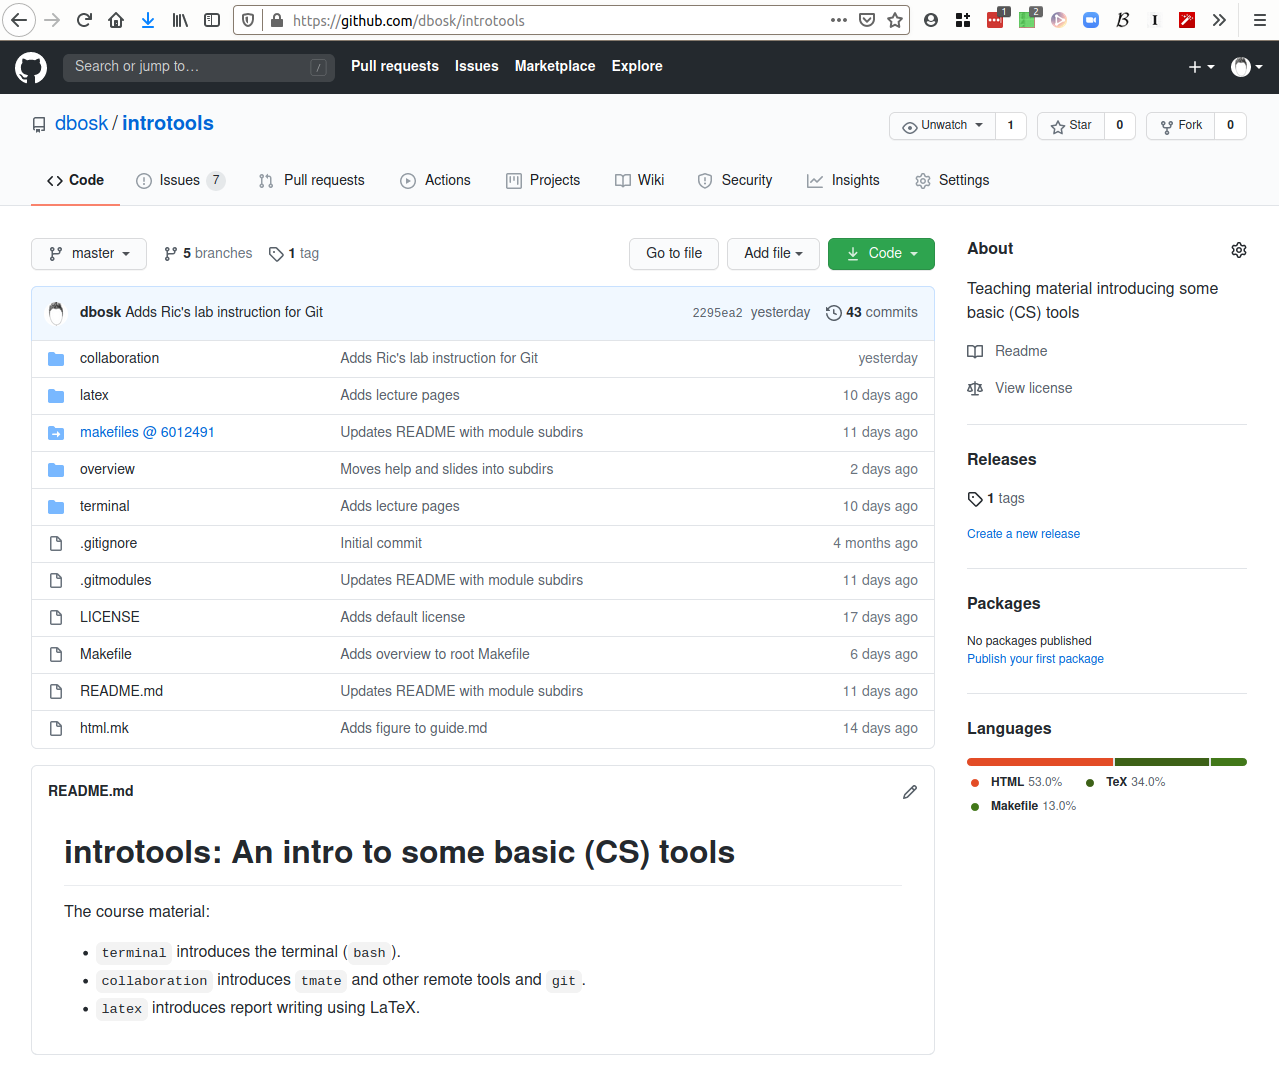
\includegraphics[height=\textheight]{figs/github-introtools.png}
\end{frame}

\subsection{Version control systems}

\begin{frame}
  \begin{block}{Centralized}
    \begin{itemize}
      \item Current version locally
      \item History remotely
    \end{itemize}
  \end{block}

  \pause

  \begin{example}
    \begin{itemize}
      \item CVS
      \item SVN
    \end{itemize}
  \end{example}
\end{frame}

\begin{frame}
  \begin{block}{Distributed}
    \begin{itemize}
      \item Current version locally
      \item History locally
    \end{itemize}
  \end{block}

  \pause

  \begin{example}
    \begin{itemize}
      \item Git
    \end{itemize}
  \end{example}
\end{frame}

\subsection{Project management}

\begin{frame}
  \begin{block}{GitHub}
    \begin{itemize}
      \item Git-repo hosting-service
      \item Issue tracker
      \item Project kanban boards
      \item All connected to the version control system
    \end{itemize}
  \end{block}
\end{frame}

%\begin{frame}
%  \centering
%  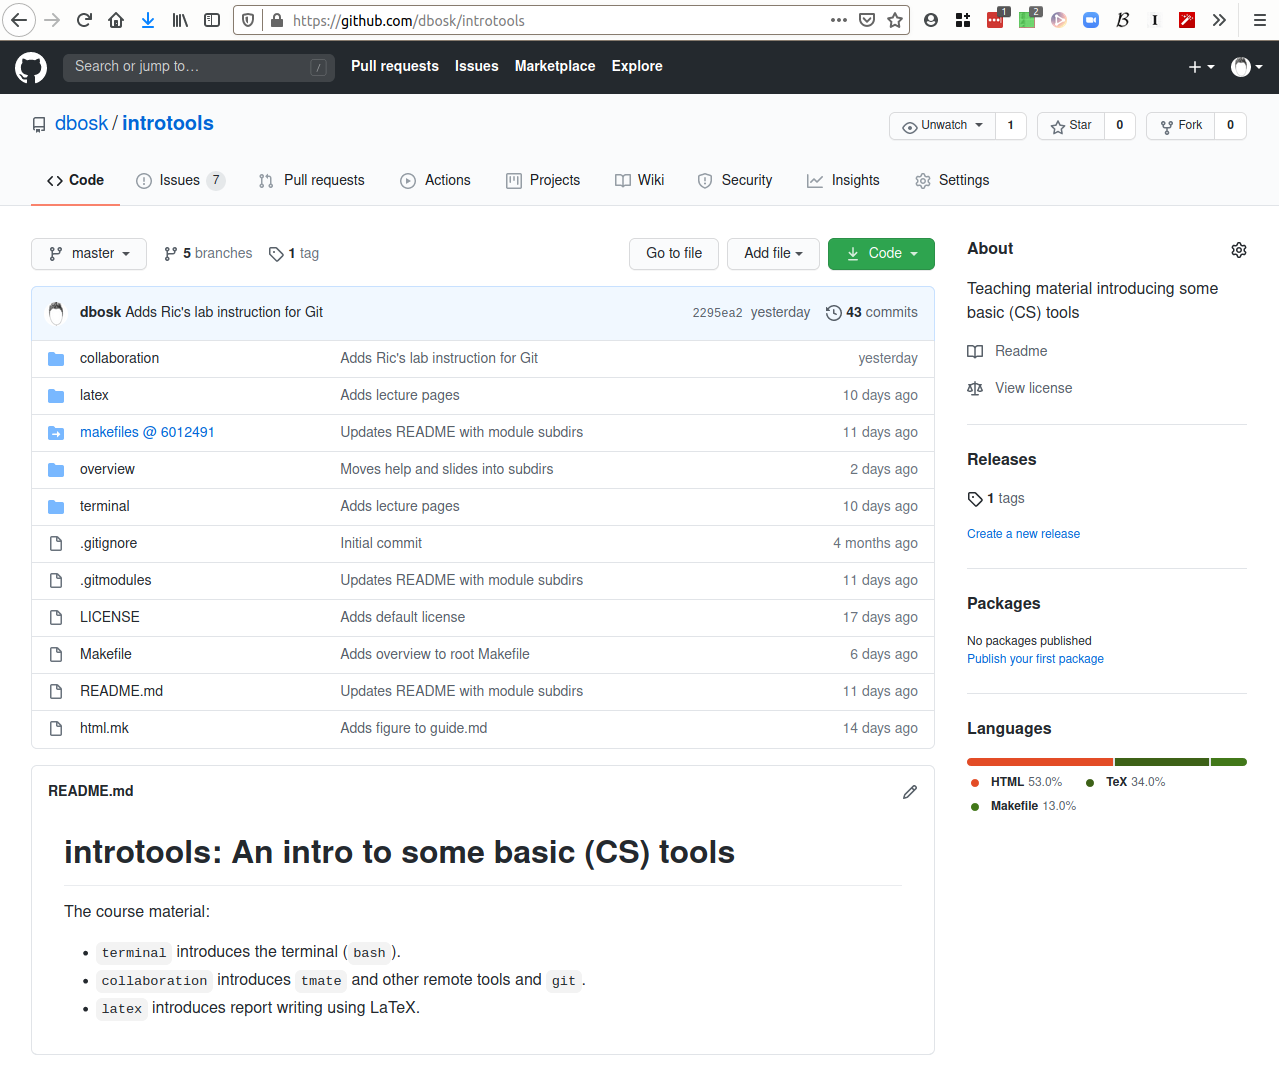
\includegraphics[height=\textheight]{figs/github-introtools.png}
%\end{frame}

\begin{frame}
  \begin{remark}
    \begin{itemize}
      \item KTH has its own instance.
      \item \url{https://gits-15.sys.kth.se}
    \end{itemize}
  \end{remark}
\end{frame}


\section{Let's get to the Git}

\subsection{Initialization}

\begin{frame}[fragile]
  \begin{example}<+>[No remote]
    \begin{lstlisting}
$ mkdir project
$ cd project
$ git init
$ vim myfile.md
[nice edits]
$ git add myfile.md
$ git commit -v
    \end{lstlisting}
  \end{example}

  \begin{example}<+>[Add remote later]
    \begin{lstlisting}
$ git remote add origin git@gits-15.sys.kth.se:datintro20/lecture-git.git
    \end{lstlisting}
  \end{example}
\end{frame}

\begin{frame}[fragile]
  \begin{example}[Most of the time]
    \begin{lstlisting}
# create repo manually in GitHub web interface
$ git clone git@gits-15.sys.kth.se:datintro20/lecture-git.git
$ cd lecture-git
    \end{lstlisting}
  \end{example}
\end{frame}

\subsection{Linear and non-linear history}

\begin{frame}[fragile]
  \begin{example}[Linear]
    \begin{lstlisting}
$ pwd
[...]/lecture-git
$ vim README.md
[nice edits]
$ git add -p
$ git commit
$ vim README.md
[make further improvements]
$ git add -p
$ git commit -v
$ git push
    \end{lstlisting}
  \end{example}
\end{frame}

\begin{frame}[fragile]
  \begin{example}[Non-linear]
    \begin{lstlisting}
$ git switch -c rewrite-README
$ vim README.md
[make some changes]
$ git add -p
$ git commit
$ git switch master
$ vim README
[fix typo]
$ git add -p
$ git commit
$ git switch rewrite-README
$ vim README.md
[continue]
$ git add -p
$ git commit
$ git push --all
    \end{lstlisting}
  \end{example}
\end{frame}

\subsection{Merging}

\begin{frame}[fragile]
  \begin{example}[Merging]
    \begin{lstlisting}
$ git switch master
$ git merge rewrite-README
    \end{lstlisting}
  \end{example}
\end{frame}

